\subsection{Task 4.3 -- MVP Sprint 1}

MVP Sprint 1 cho phép khách mở web trên điện thoại, xem menu và mở chi tiết món
từ dữ liệu do API cung cấp. \texttt{GET} \nolinkurl{/api/products} trả danh sách
món và hỗ trợ lọc theo danh mục. \texttt{GET} \nolinkurl{/api/products/:id} trả
chi tiết theo mã món và trả HTTP 404 nếu mã không tồn tại.
Hai endpoint nằm trong \nolinkurl{products.controller.ts} của module sản phẩm.

Trang chủ Next.js hiển thị danh sách món qua \texttt{AllDrinksScroll}. Màn hình
có trạng thái tải, thông báo khi danh sách rỗng và thông báo lỗi khi tải thất
bại. Khi có dữ liệu, khách có thể chọn món để mở trang
\nolinkurl{/product/[id]}. Prisma seed và các script tạo danh mục, nạp tồn demo
chuẩn bị dữ liệu trên PostgreSQL local theo \nolinkurl{docker/README.md}.

Ở bộ kiểm thử hiện tại, \nolinkurl{AllDrinksScroll.spec.ts} kiểm tra các trạng
thái của menu. \nolinkurl{app.e2e-spec.ts} gọi API menu và chi tiết món trước
khi đi tiếp đến luồng đặt đơn. Các lệnh chạy và dữ liệu kiểm thử được ghi tại
\nolinkurl{tests/README.md}.

\paragraph{Minh chứng giao diện menu}
Các ảnh dưới đây được chụp trực tiếp từ web production ngày 20/11/2026,
với phiên khách chưa đăng nhập. Đây là minh chứng hiện tại cho các chức năng
menu và chi tiết món thuộc phạm vi MVP Sprint 1. Ảnh không thay thế kết quả
kiểm thử API hoặc ghi nhận thời điểm hoàn thành sprint.

\begin{reportfigure}
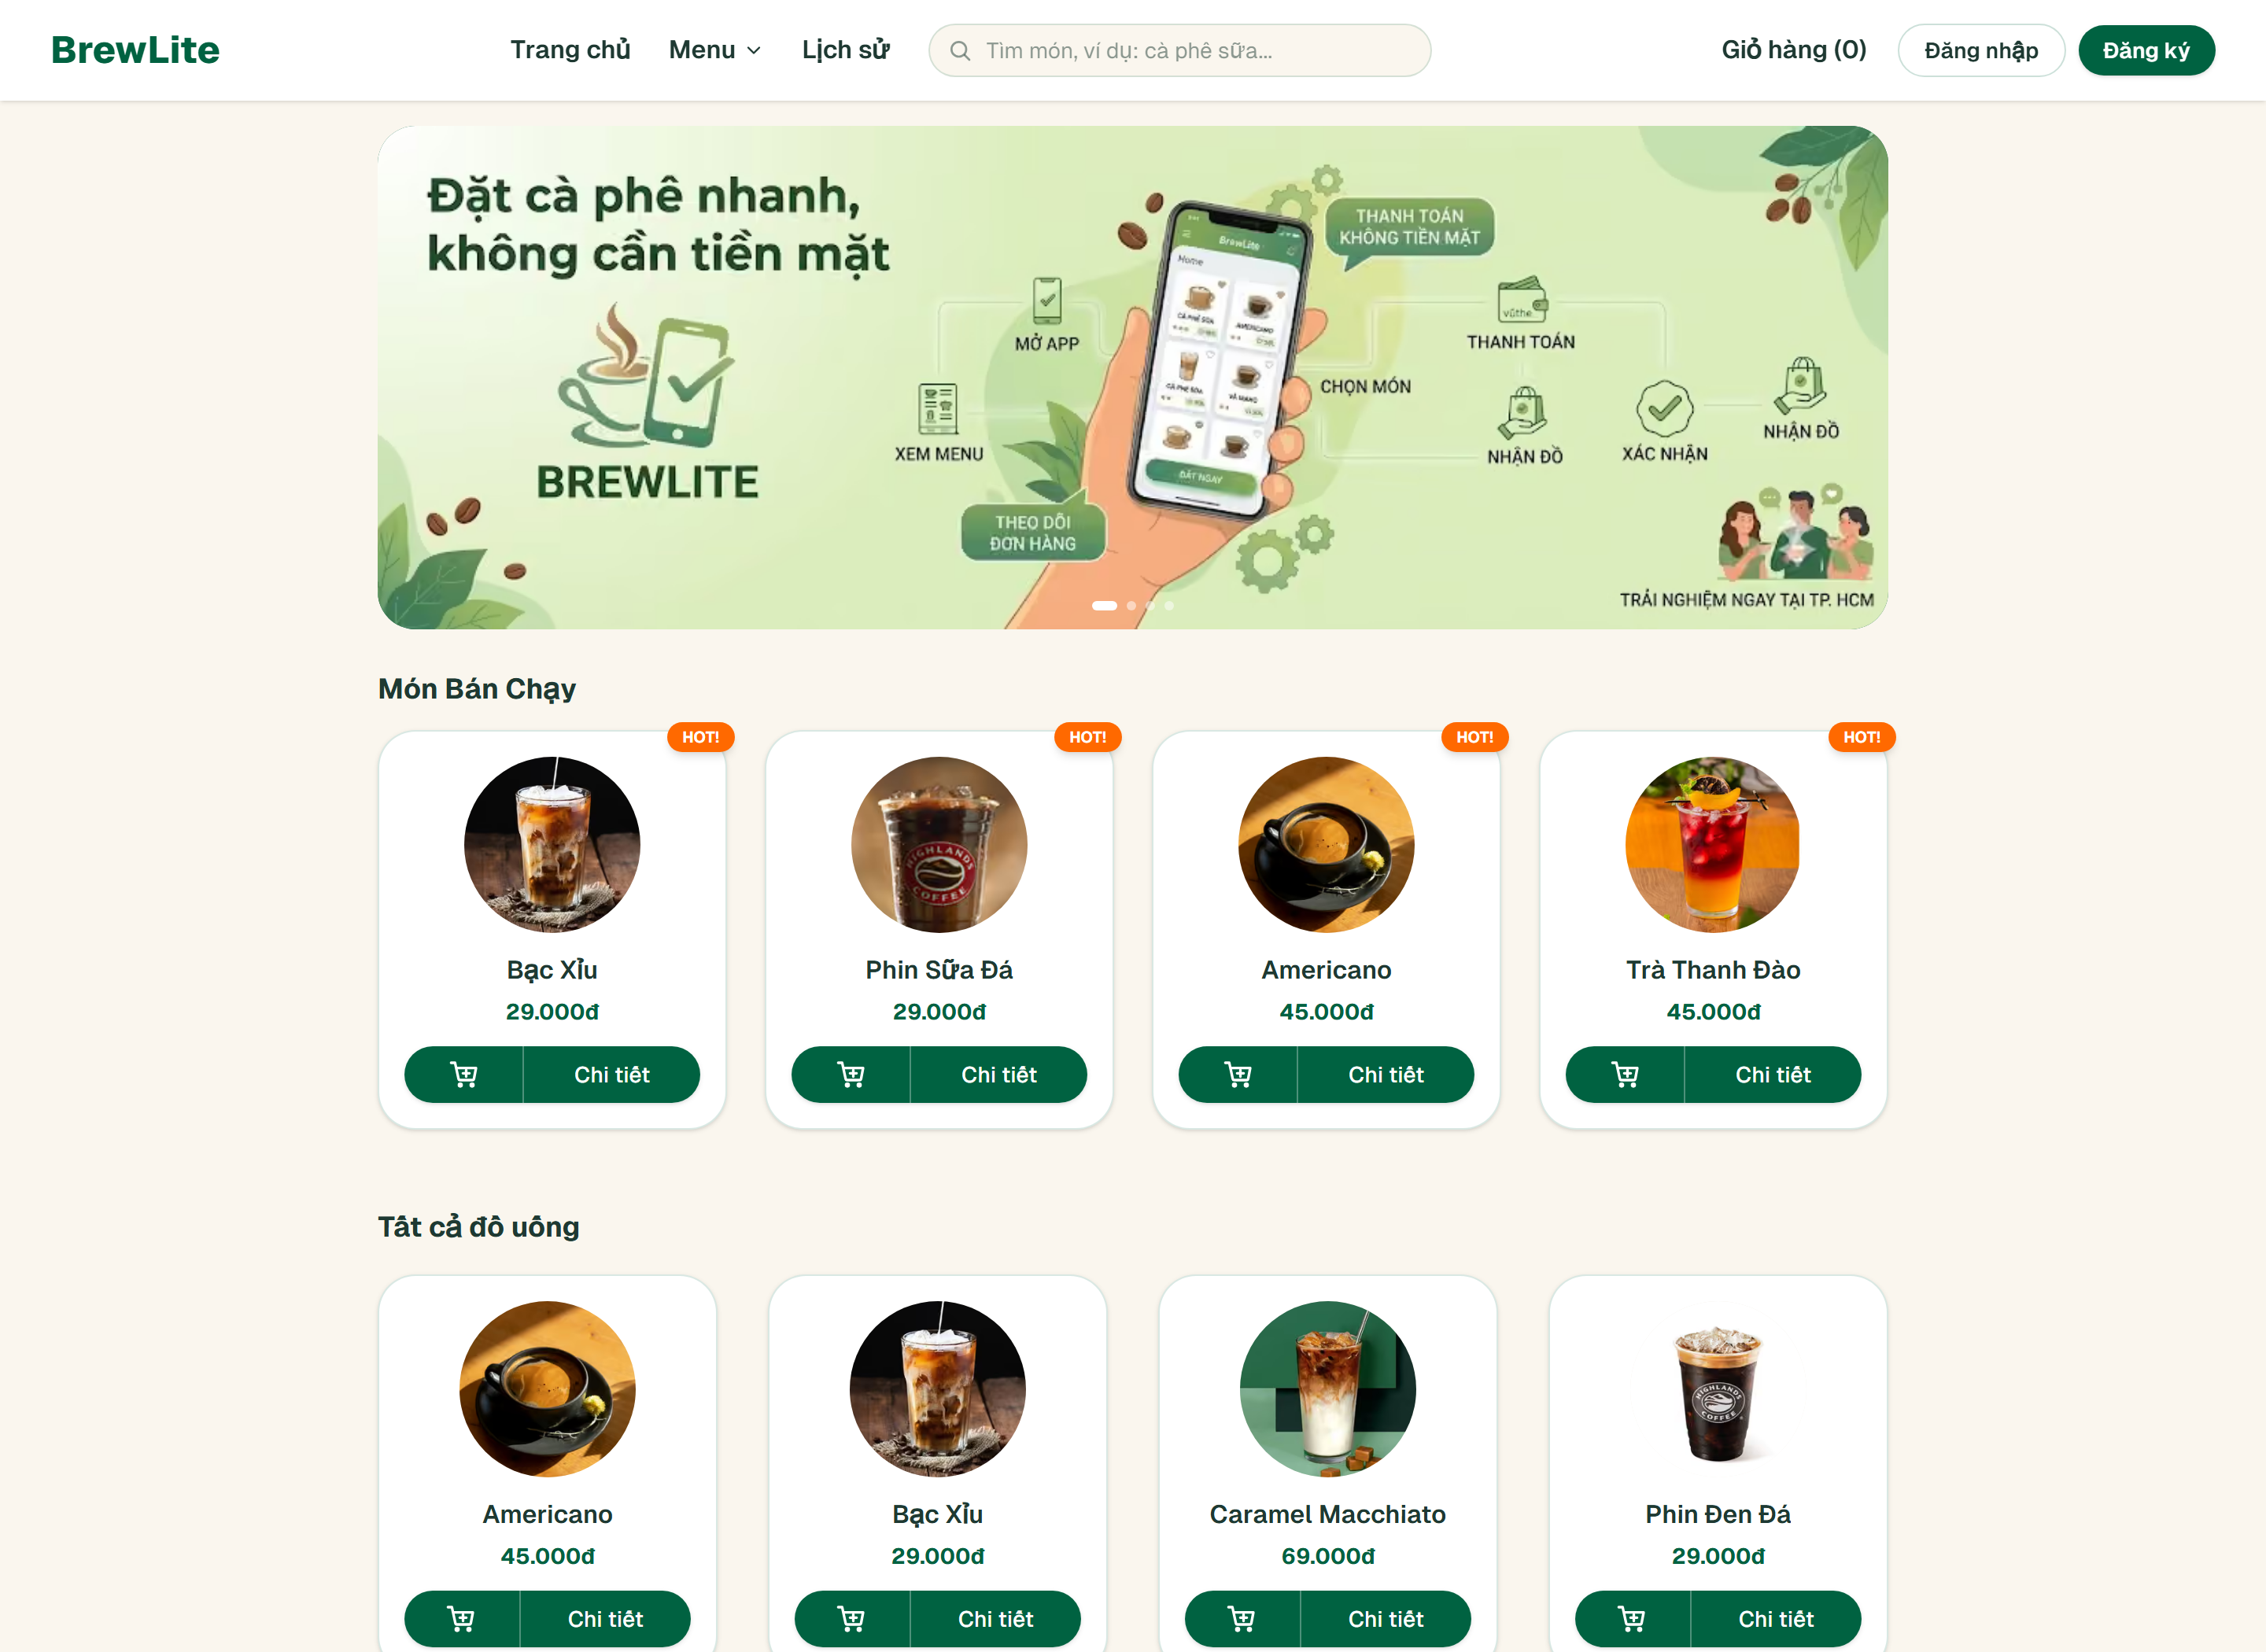
\includegraphics[width=\linewidth,height=.66\textheight,keepaspectratio]{../../assets/evidence/mvp-menu-desktop.png}
\par\small\itshape Hình 4.3a. Menu trên desktop: món bán chạy, danh sách đồ uống,
giá và liên kết mở chi tiết món
\end{reportfigure}

Khách có thể mở chi tiết từ thẻ món. Danh sách món được tải từ API; ảnh chụp
ghi nhận dữ liệu hiển thị trên production tại thời điểm thu thập.

Trang chi tiết hiển thị tên món, mô tả, giá và các lựa chọn size, số lượng,
tổng tiền tạm tính cùng thao tác thêm vào giỏ. Màn hình minh họa đường đi
từ menu đến \nolinkurl{/product/[id]}; các chức năng giỏ hàng và thanh toán
được trình bày tiếp ở MVP Sprint 2.

Ảnh được chụp bằng trình duyệt mô phỏng kích thước điện thoại. URL, viewport
và thời điểm chụp được lưu trong \nolinkurl{docs/assets/evidence/ui-capture.json}.

\paragraph{Minh chứng chi tiết món và giao diện điện thoại}\leavevmode\par\nobreak
\begin{reportfigure}
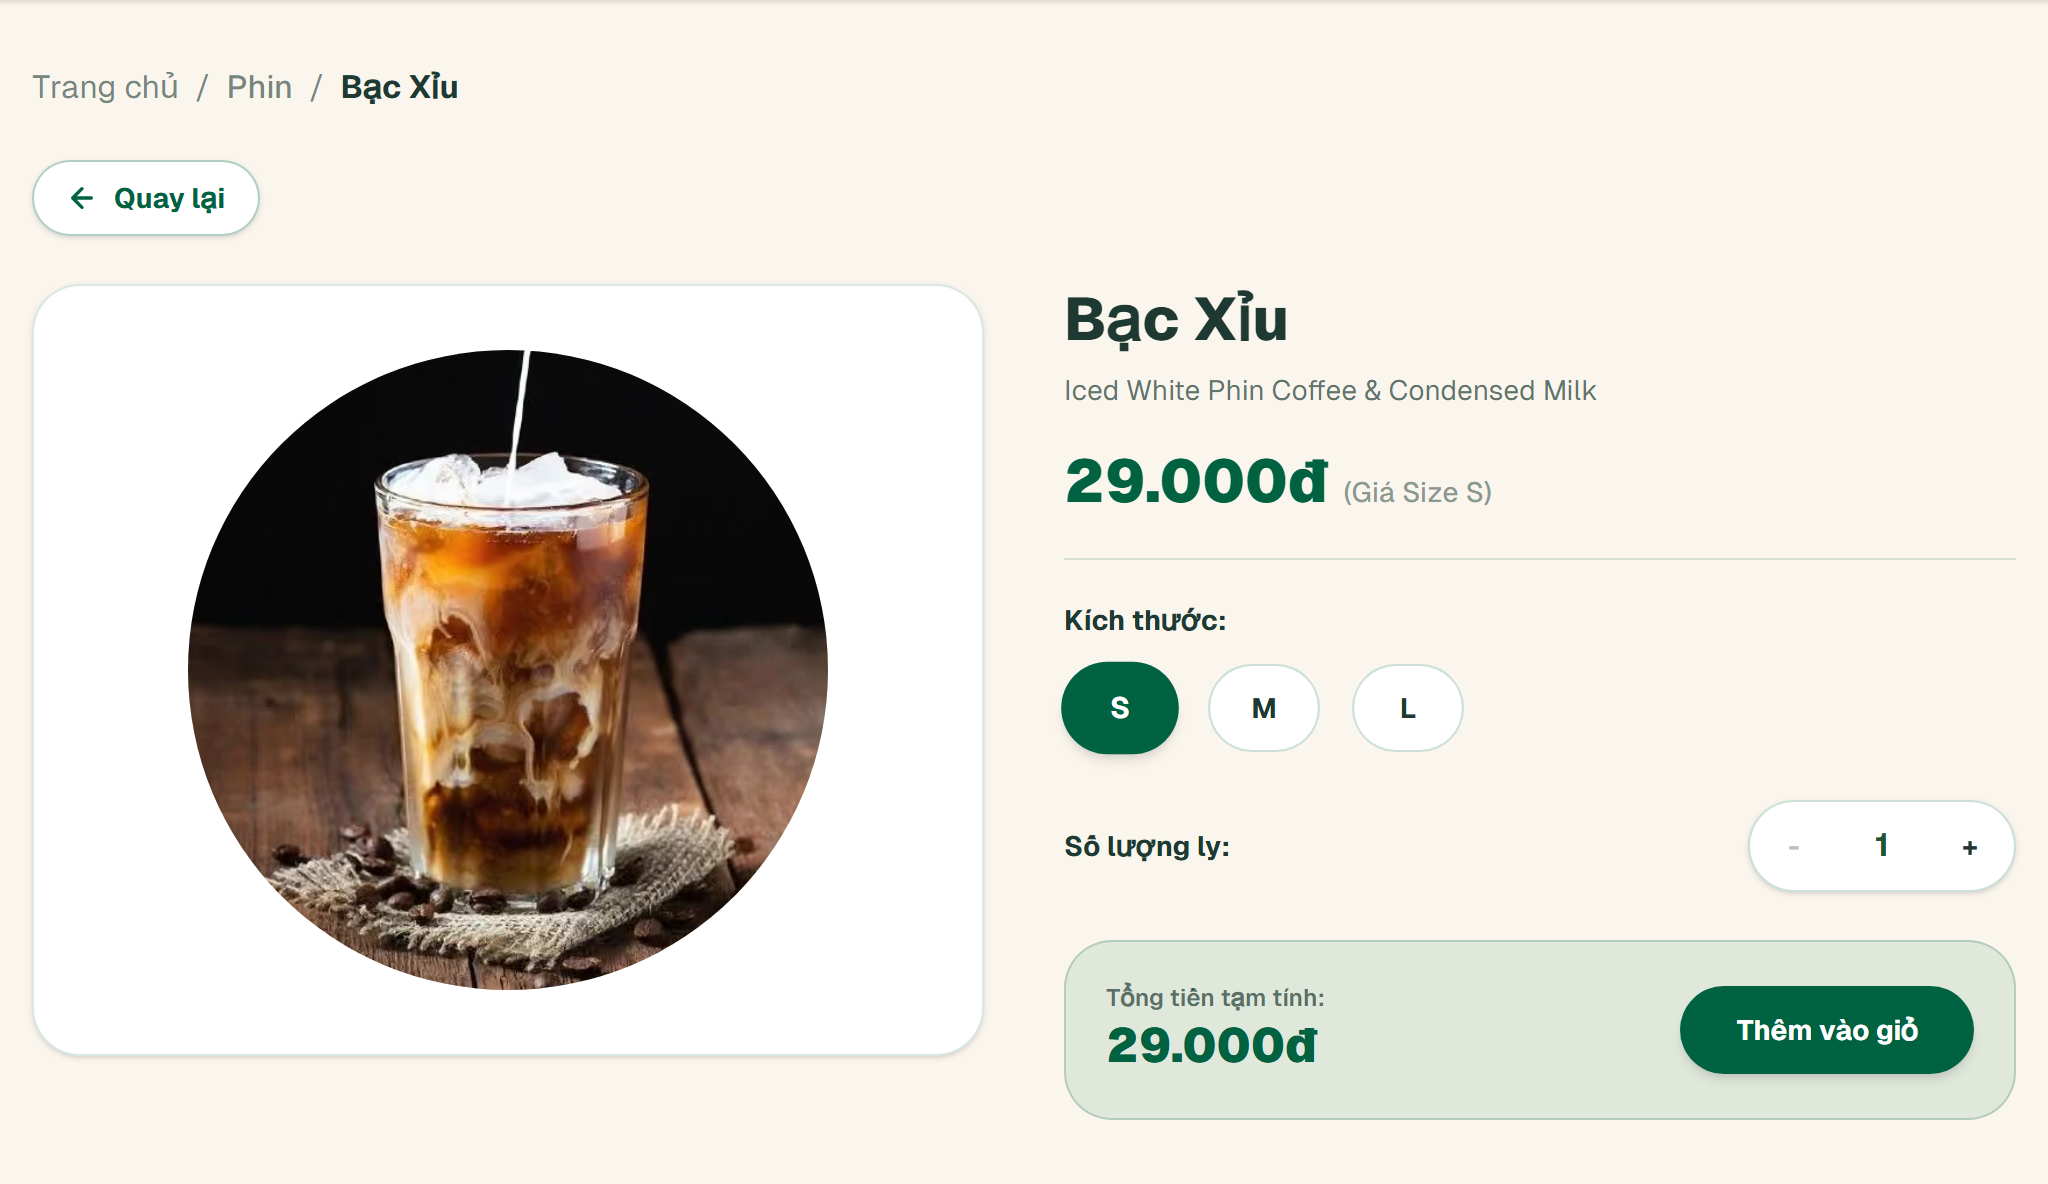
\includegraphics[width=\linewidth,height=.68\textheight,keepaspectratio]{../../assets/evidence/mvp-detail-desktop.png}
\par\small\itshape Hình 4.3b. Trang chi tiết Bạc Xỉu trên desktop
\par\medskip\normalfont\normalsize
\begin{minipage}[t]{.48\linewidth}
  \vspace{0pt}\centering
  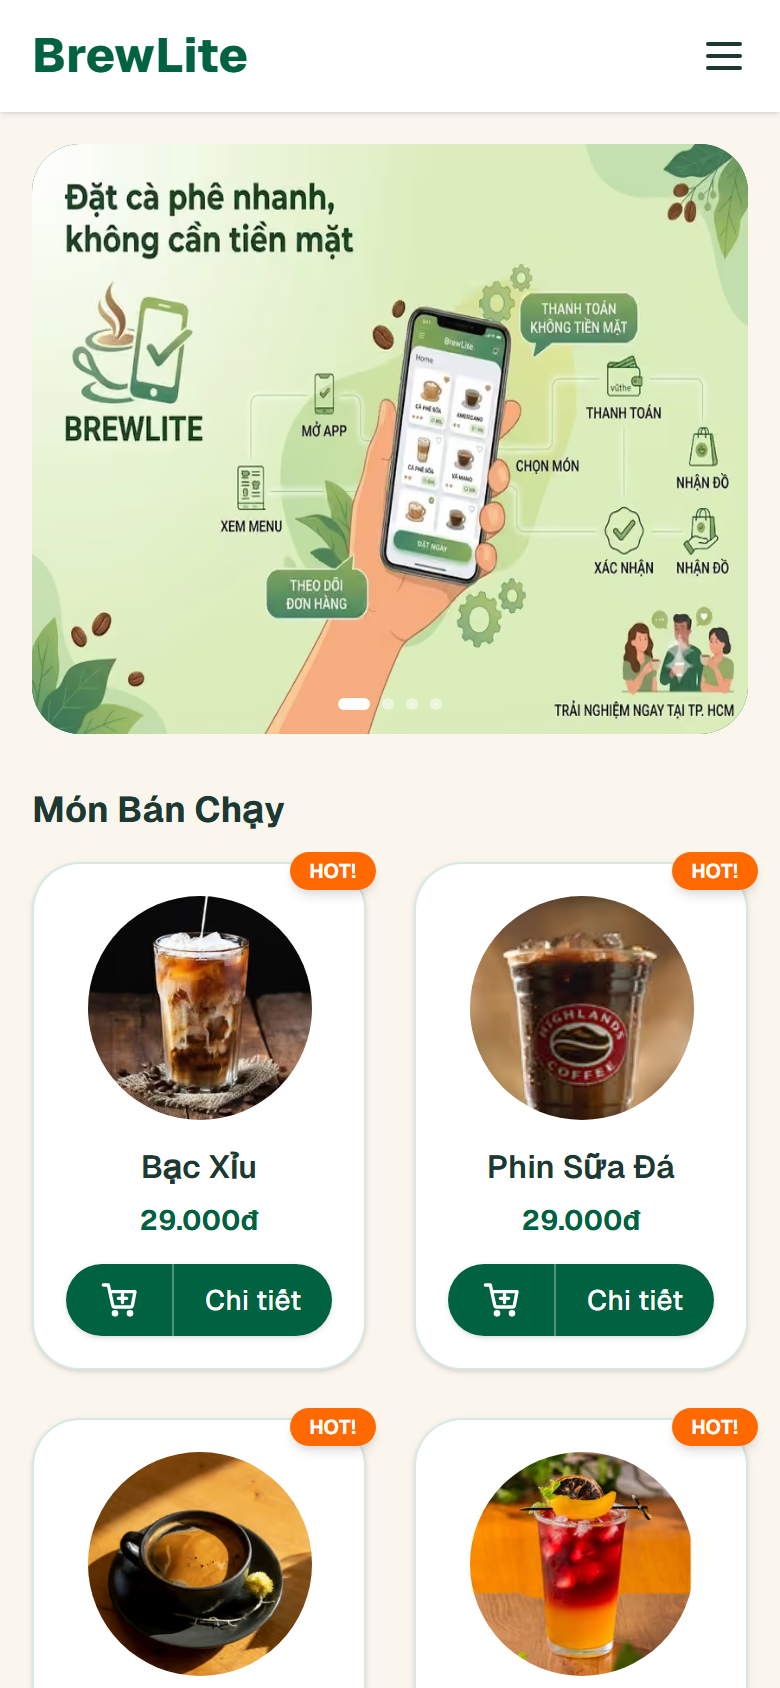
\includegraphics[width=\linewidth,trim=0bp 0bp 0bp 760bp,clip]{../../assets/evidence/mvp-menu-mobile.png}
  \par\small\itshape Menu
\end{minipage}\hfill
\begin{minipage}[t]{.46\linewidth}
  \vspace{0pt}\centering
  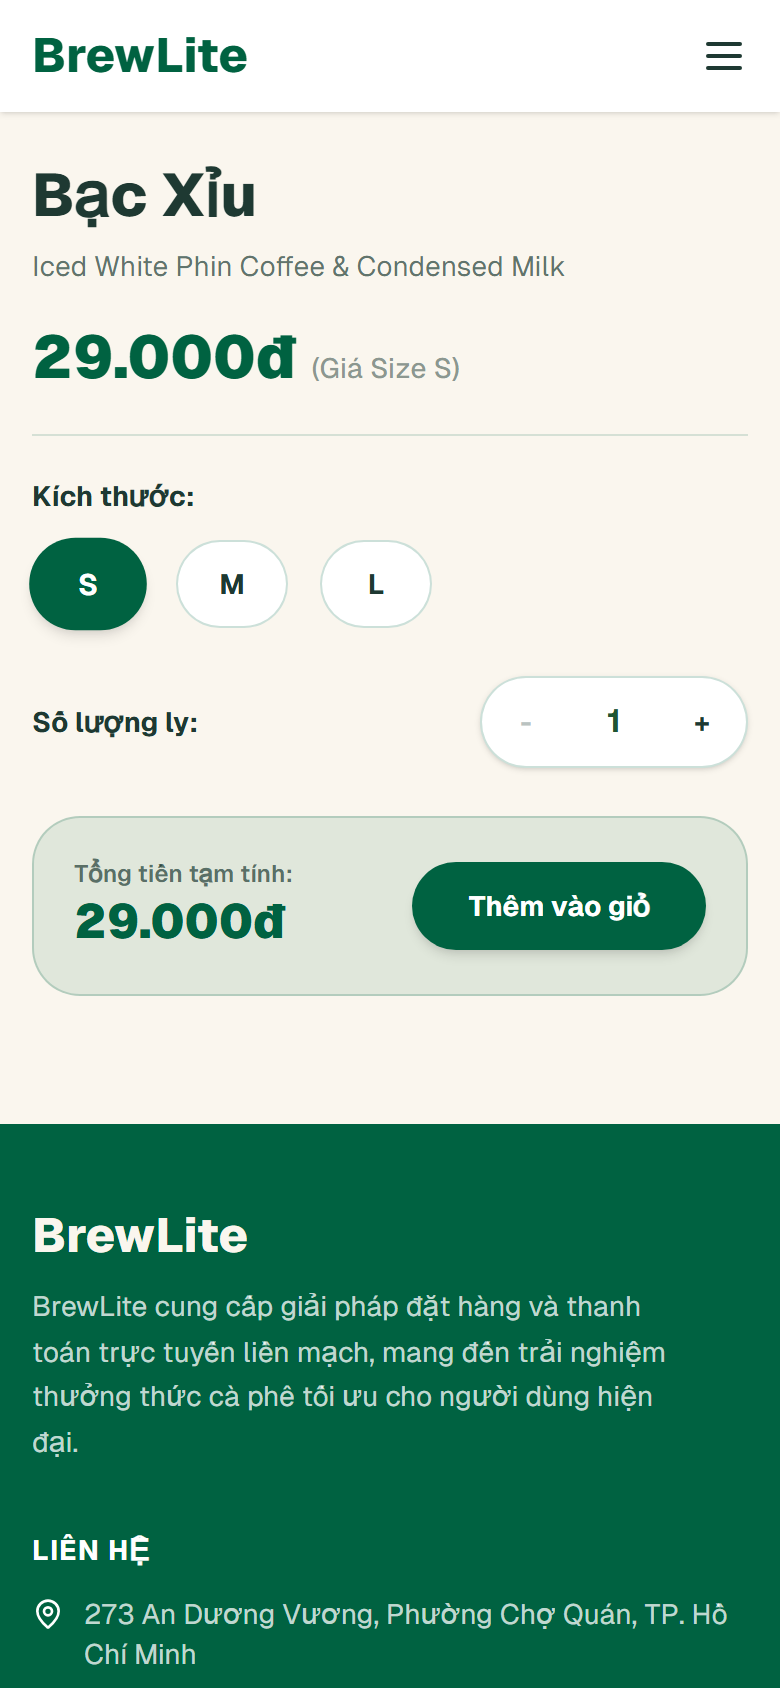
\includegraphics[width=\linewidth,trim=0bp 580bp 0bp 130bp,clip]{../../assets/evidence/mvp-detail-mobile.png}
  \par\small\itshape Chi tiết món
\end{minipage}
\par\small\itshape Hình 4.3c. Trích vùng menu và tùy chọn món ở viewport 390 $\times$ 844 px
\end{reportfigure}
